\section{超引力中的暴胀模型简介}
在超引力中嵌入暴胀模型的研究已经超过三十年了,第一个在超引力中实现的暴胀模型——
混沌暴胀可追溯之1983年
\citep{goncharov1984chaotic},与混沌暴胀的一般化模型的提出仅相隔几个月。 
这一章论述在超引力中利用平移对称性构造跑动动能暴胀模型,并以此为出发点对场进行
正则归一化,从而得到符合拐点暴胀模型的势能函数。

早期超引力暴胀模型通常涉及多个手征多态。例如,有一类双场理论
\citep{kallosh2010new,kallosh2010new},$S=s
e^{i\theta}/\sqrt{2}$和$\Phi=(\phi+i\chi)/\sqrt{2}$,以及超势$W=Sf(\Phi)$,其中$f(\Phi)$是实全纯函数,满足$\bar{f}(\Phi)=f(\Phi)$。
模型中有两个超场,或者四个实标量场,$s$,$\theta$,$\phi$和$\chi$,其中只有
一个实场对应暴胀场,参与宇宙学演化。通常选取$\phi$或$\chi$作为暴胀场,$S$作为辅助场,
为了避免势能出现指数爆炸的情形,K\"ahler势的函数形式可以取做$K=K({(\Phi-\bar{\Phi})}^2,S\bar{S})$。这种情形下,势能$V$在$s=\chi=0$处有极值,如果该极值同时也
是全局最小值,那么标量场$\phi$将扮演正则归一化的暴胀场,势能为$V(\phi)=|f(\phi/\sqrt{2})|^2$,且暴胀过程发生在$s=\chi=0$的方向上。为了与宇宙学观测保持一致,
暴胀模型需要给出符合观测的宇宙学参数$n_{s}$和$r$,这一点总是可以通过选取合适
的函数$f(\Phi)$来做到。在某些模型中,需要特别注意辅助场$S$在$s=0$处的稳定性。
有两种方法可以做到,一是在K\"ahler势中添加项$S\bar{S}$,二是选择不含标量自由度
的手征场$S$作为辅助场。后一种方法中涉及描述宇宙演化的只有一个无约束的手征超场$\Phi$场。
基于此,产生了一类无需引入额外非约束手征超场就能描述当前宇宙演化的暴胀模型
\citep{kallosh2015inflation,dall2014sgoldstino,linde2015does} 。

后来,Ketov和Terada提出了一类基于单手征超场$\Phi$的新暴胀理论
\citep{ketov2014generic,ketov2014inflation}。在 \citep{ketov2014generic}
中,提出了一种新的对数形式的K\"ahler势
\begin{equation}
  \label{eq:logarithmic-kahler-potential}
  K =
-3\left[1+\frac{\Phi+\bar{\Phi}+\zeta{\left(\Phi+\bar{\Phi}\right)}^{4}}{\sqrt{3}}\right].
\end{equation}
$\zeta$是常系数。不论超势取何种形式,当K\"ahler势取$(\ref{eq:logarithmic-kahler-potential})$式时,场$\Phi$的动能项系数为
\begin{equation}
  \label{eq:kinetic-coefficient-of-Phi}
  G(\phi,\chi) =
  \frac{3(1+32\zeta^2\phi^{6}-8\zeta\phi^2(3\sqrt{3}+\sqrt{2}\phi))}{{\left(\sqrt{3}+\sqrt{2}\phi+4\zeta\phi^{4}\right)}^2}.
\end{equation}

\begin{figure}[!http]
  \centering
  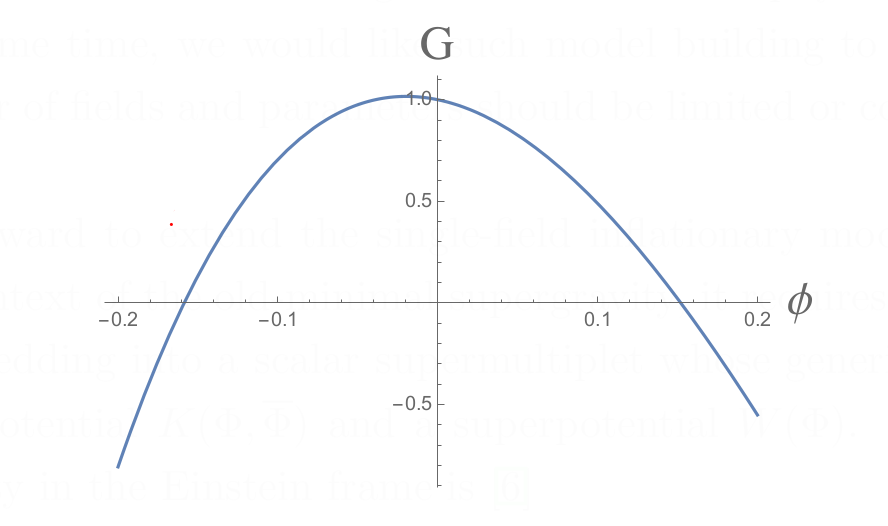
\includegraphics{Img/kinetic_coefficient_for_Phi.png}
  \caption{$\zeta=1$时,手征场$\Phi$的动能项系数与$\phi$的函数关系}\label{fig:kinetic-coefficient_for_Phi}
\end{figure}

从图$(\ref{fig:kinetic-coefficient_for_Phi})$可知,为了使$G>0$,$\phi$被限制在一
个有限的区间内。$\zeta$越大,$\phi$的取值区间越窄。因而在暴胀期间,标量场$\phi$的影响可以忽略,势能近似为暴胀场$\chi$的函数,当超势为
\begin{equation}
  W = \frac{1}{\sqrt{2}} f(-\sqrt{2}i\Phi),
\end{equation}
时,其中$f$为实函数,延暴胀场方向的势能为
\begin{equation}
  V\simeq {\left[f^\prime(\chi)\right]}^2.
\end{equation}
暴胀结束后,场朝着全局最小值滚去,最终得到一个超对称闵可夫斯基真空。为了能够
描述真实的宇宙,暴胀结束后应该得到一个真空能约为$V_0 \sim
10^{-120}$的德$\cdot$西特宇宙。根据no-go定理,必须引入额外的手征超场作为超对称
破缺项,并抬高真空能使得暴胀结束后能得到一个德$\cdot$西特真空。在引入额外超场
后,暴胀演化将涉及多个标量场,除非额外场被稳定在极值处\citep{dudas2013strong} 
或者属于零幂手征多态
\citep{ferrara2014cosmology,kallosh2015inflation,dall2014sgoldstino,linde2015does}。

其次是\textbf{跑动动能暴胀}模型,是指场的质量在暴胀期间会随场的变化而变的模型
。对于慢滚暴胀模型,习惯假设暴胀场是弱耦合场,其拉氏量中的动能项在暴胀期间及暴
胀结束后不会发生大的改变。又为了暴胀能够产生,通常利用对称性产生平坦的势能。如
果不利用对称性,通常需要精细调节参数来获得平坦的势能,且需要挑选能够使暴胀发生
的初始位置。后来,有人提出了一类新的暴胀模型,丢弃了动能项的变化被忽略的假设。
在整个暴胀期间,动能项的变化不能被忽略,在某些情况下,这种变化甚至能明显地影响
到暴胀场的动力学。这样的模型被称为\textbf{跑动动能暴胀}模型。

\textbf{出发点} 

假设实标量场$\phi$有如下形式的拉氏量,
\begin{equation}
  \mathcal{L} =
  \frac{1}{2}f(\phi)\partial^{\mu}\phi\partial_{\mu}\phi-V(\phi),
\end{equation}
假设场$\phi$在某个区间时,$f(\phi)$的行为能够近似为$f(\phi)\approx
\phi^{2n-2}$,$n$为给定的整数。则对场$\phi$作正则归一化之后,$\hat{\phi}\equiv
\phi^{n}/n$,势能函数将会变得更加平坦。例如,当$n=2$时,二次(四次)方势能函数,$V(\phi)\propto
\phi^2(\phi^{4})$,将变成线性(二次)势能$V(\hat{\phi})\propto
\hat{\phi}(\hat{\phi}^2)$。因此暴胀场的动力学非常依赖其动能项。

再举一个例子,
\begin{equation}
  f(\phi) = \kappa + \phi^2. 
\end{equation}
其中$0 < \kappa \ll 1$。因此当$\phi \gtrsim \sqrt{\kappa}$时,$f(\phi)
\approx \phi^2$。当$\phi \ll \sqrt{\kappa}$时,$f(\phi)\approx
\sqrt{\kappa}$。因此,标量场$\phi$将按如下方式进行正则归一化
\begin{equation}
  \hat{\phi} = 
  \begin{cases}
    \frac{\phi^2}{2}, \qquad & \phi \gg \sqrt{\kappa} \\
    \sqrt{\kappa},\qquad & \phi \ll \sqrt{\kappa}
  \end{cases},
\end{equation}
故而当$V(\phi)=m^2\phi^2/ 2$时,正则场的势能函数为
\begin{equation}
  V(\hat{\phi}) \simeq 
  \begin{cases}
    m^2\hat{\phi},\qquad & \hat{\phi} \gg \kappa \\
    \frac{m^2}{2\kappa} \hat{\phi}^2,\qquad & \hat{\phi} \ll \kappa
  \end{cases}.
\end{equation}
从这个例子可以发现,从一个形式简单的拉氏量出发,经过正则归一化,能够轻松实现势能
函数从线性形式到二次函数的转变。
原则上,我们可以把正则场$\hat{\phi}$满足的拉氏量作为出发点,得到的暴胀模型拥有
相同的动力学。然而,这种方式难以从理论上解释为何暴胀场的势能取这样一种特定的函数
形式。


